\documentclass{ctexart}
\usepackage{bookmark}
\usepackage{amsmath}
\usepackage{graphicx}
\usepackage{pgfplots}
\usepackage{xcolor}
\usepackage[all,pdf]{xy}
\usepackage{listings}
\usepackage{minted}
\usepackage{import}

\lstset{
  language         = C,
  frame            = single,
  numbers          = left,
  tabsize          = 4,
  showstringspaces = false,
}
\newcommand{\mdcode}[1]{\texttt{\colorbox{lightgray}{#1}}}

\title{并行程序设计实验报告}
\author{}
\date{}

\begin{document}
\maketitle
\tableofcontents
\newpage
\section{实现}
\subsection{遇到的问题与解决措施}
\subsubsection{问题}
提供的CYK算法的串行实现代码中,使用到了\mdcode{subTreeBuf}用来保证二维表中
的子树索引的有序性,该部分在使用openmp或者pthread处理时会导致数据竞争,需
要修改。
\subsubsection{解决措施}
CYK算法不断填充字符串长度作为长宽的二维表格,表格中的(i, j)单元表示子字符串
(i, j)对应的子树,填充过程中,子串长度为n-1的单元格依赖于子串长度为n的单元
格。

依赖关系如下图,$\xymatrix{ X\ar[r] & Y }$表示$Y$依赖于$X$的完成。

\begin{figure}[h]
  \centering
  \xymatrix{
    (1, 1)\ar[r] & (1, 2)\ar[r]       & (1, 3)\ar[r]       & (1, 4)\ar[r]       & (1, 5)       \\
                 & (2, 2)\ar[r]\ar[u] & (2, 3)\ar[r]\ar[u] & (2, 4)\ar[r]\ar[u] & (2, 5)\ar[u] \\
                 &                    & (3, 3)\ar[r]\ar[u] & (3, 4)\ar[r]\ar[u] & (3, 5)\ar[u] \\
                 &                    &                    & (4, 4)\ar[r]\ar[u] & (4, 5)\ar[u] \\
                 &                    &                    &                    & (5, 5)\ar[u] \\
  }
  \caption{依赖关系图}
  \label{fig:dep}
\end{figure}

单元格中需要记录当前子树可用的产生式左部以及对应数量,该部分使用类似链
表的结构(通过数组实现)进行记录。其中`number'记录该单元格含有多少个产生式
左部,数组中的剩余元素为相应的产生式左部。

\begin{center}
\xymatrix{
  *+=[o][F]{number}\ar[r] & *+[F]{val0}\ar[r] & *+[F]{val1}\ar[r] & *+[F]{val2}\ar[r] & \ldots 
}
\end{center}

`valx'是否需要添加到链表中只需要根据对应的语法树数量是否为0确定。

该部分结构在代码中通过\mdcode{table\_list}实现,以下是使用\mdcode{table\_list}
填充单元格的代码。

% \begin{lstlisting}[caption={单元格计算-0}, label={lst:code0}]
\begin{minted}[frame=lines,linenos]{c}
for (k = i; k <= j - 1; ++k) {
  p_range = table_list[i][k][0];
  q_range = table_list[k + 1][j][0];
  for (p = 1; p <= p_range; ++p) {
    for (q = 1; q <= q_range; ++q) {
      B = table_list[i][k][p];
      C = table_list[k + 1][j][q];

      if (vn_index[B][C].end != vn_index[B][C].start) {
        BC_num = table_num[i][k][B] * table_num[k + 1][j][C];
        left = vn_index[B][C].start;
        right = vn_index[B][C].end;
        for (binary_index = left; 
              binary_index < right;
              ++binary_index) {
          A = binaries_parent[binary_index];
          if (!table_num[i][j][A]) {
              table_list[i][j][0]++;
              table_list[i][j][table_list[i][j][0]] = A;
          }
          table_num[i][j][A] += BC_num;
        }
      }
    }
  }
}
\end{minted}
% \end{lstlisting}

其中\mdcode{p\_range}与\mdcode{q\_range}分别为$A\rightarrow BC$中有多少个
$B,C$的数量。

当计算单元格设计到较多产生式时,由于上述算法包含条件判断,不利于流水线执行,
所以采取如下方法。

\begin{lstlisting}[caption={单元格计算-1}, label={lst:code1}]
for (k = i; k <= j - 1; ++k) {
  for (p = 0; p < binary_production_number; ++p) {
    B = binaries[p].left;
    C = binaries[p].right;
    A = binaries[p].parent;
    table_num[i][j][A] += table_num[i][k][B] 
                          * table_num[k + 1][j][C];
  }
}
\end{lstlisting}

将内层寻找B与C的两重循环修改为直接遍历所有二元产生式的一重循环,不再记录子
树索引,而是直接计算子树数量。

\subsection{任务分块}

任务分块时,一个线程处理一个固定长度的子串,即一个线程处理二维表格中的斜对
角线上的所有单元格,线程每处理完一个单元格后,子串长度比其小1的线程就可以运行。

以上文中的\hyperref[fig:dep]{依赖关系图}为例,输入字符串长度为5,总共创建
5个线程,线程间通过信号量进行通信。

\begin{itemize}  
  \item
    线程1处理:(1, 1), (2, 2), \ldots, (5, 5)
  \item
    线程2处理:(1, 2), (2, 3), (3, 4), (4, 5)
  \item
    \ldots
  \item
    线程5处理:(1, 5)
\end{itemize}

当线程1处理完(1, 1)与(2, 2)后,线程2就可处理(1, 2)单元格。在子串长度更长的
线程没有完成相应任务时,当前线程处于休眠状态,当唤醒的线程数量多于操作系统
可用的线程数量时,线程的调度由操作系统完成。在代码的执行过程中,程序的并行
性会逐步增加。

\begin{lstlisting}[caption={单个线程任务}, label={lst:routine}]
void *routine(void *aux) {
  int thread_num = (int)aux;
  int i;
  void (*f) (int, int, void *);
  f = (s_len > MAX_STRING_LENGTH * 4 / 5) ? 
      sub_str_process_v0 : sub_str_process_v1;

  for (i = 0; i < s_len - thread_num; ++i) {
    sem_wait(&sems[thread_num]);
    f(i, i + thread_num, aux);
    if (i != 0 && thread_num != s_len - 1)
      sem_post(&sems[thread_num + 1]);
  }
  return NULL;
}
\end{lstlisting}

以上为单个线程需要执行的任务,函数\mdcode{f}为在单个单元格上执行的操作,观
察发现,三份输入样例的数据特点不同,所以\mdcode{f}会相应地调用不同的计算操
作。

\subsection{运行速度提升与程序扩展性增强}
程序运行速度提升可分为以下几部分:
\begin{itemize}
  \item
    多线程处理任务。

    通过使用pthread线程库,将原本的串行执行代码并行化,充分
    利用多核处理机的计算能力。
  \item
    不同的任务划分方式。

    最初的代码并行化实现时,采用openmp在计算相同长度的
    子串时进行并行化处理,即将斜对角线上的任务并行化,其实质是在对角线上创
    建不同的线程,最后依靠屏障完成同步,当子串长度越来越大时,多核处理机的
    算力无法充分发挥,并且存在的显著问题是不同子串长度的线程无法同时运行,
    openmp封装操作的同时就失去了针对特定任务的调整能力。

    现行的做法是使用pthread手动划分任务,不同子串长度的线程可以同时运行,通
    过信号量保证数据的一致性,当子串长度更小的线程处理完单个单元格后,子串
    长度大1的线程就可被唤醒执行,并且在程序执行的过程中,越来越多的线程可参
    与执行,并行程度逐步增加并保持稳定,详见\hyperref[lst:routine]{Listing\ 3}。
  \item
    遍历产生式右部的选取方式。

    对于产生式$A\rightarrow BC$,选取可用的$B,C$时,使用链表,即可一次遍历
    完成,在创建该链表时,只需根据生成的产生式数量是否为0将其添加到链表中,
    保证了链表中元素的唯一性,减少了不必要的遍历操作,详见
    \hyperref[lst:code0]{Listing\ 1}。
   \item
      针对特殊数据分布的优化。

      对于计算单元格中的产生式左部可能会用到较多二元产生式的数据时,使用链
      表结构会减慢速度,因为每次加入链表中的元素大概率是新出现的,会导致较
      多的if条件判断和重复的对产生式左部元素数量的增加。因此,将二重循环改
      为一重循环,直接遍历所有的产生式,只进行数据相乘与累加操作,该方法在
      需要使用较多产生式推导的样例中表现更好,详见\hyperref[lst:code1]{Listing\ 2}。
    \item
      局部变量外提。

      代码中有大量嵌套循环,将在每次循环内创建的变量提至循环最外层,减少变
      量创建的开销,在hpc平台的gcc默认c89(或者是gnu89)编译环境下有显著效
      果。

    \item
      开启编译器优化。

      在代码开头加上编译器优化指令\mdcode{\#pragma\ GCC\ optimize("Ofast")},
      借助编译器的优化功能实现代码中的优化。

\end{itemize}
程序扩展性通过创建多个的线程数量等于字符串长度实现,由于输入字符串长度
一般远大于可用线程数,所以在程序的运行后期,CPU能够得到充分利用。

\section{分析与实验}
\subsection{测量程序运行时间}
由于是并行程序,所以程序运行时间主要体现为墙钟时间,一是可通过\mdcode{time}
指令测量,测量指令为\mdcode{sun -p cpu68 -n 1 -c 16 time -v ./a.out},可以
测量可执行程序提交到计算节点后运行的时间。
二是通过在代码中加入\mdcode{gettimeofday}函数,将程序算得结果后的时间和开始
时的时间作差得出墙钟时间。此处选用第二种方法,更为准确。

\begin{lstlisting}[caption={计算运行时间}]
int main() {
  struct timeval base_tv;
  struct timeval eval_tv;
  struct timeval res_tv;
  gettimeofday(&base_tv, NULL);
  // ...
  // ... 
  gettimeofday(&eval_tv, NULL);
  timersub(&eval_tv, &base_tv, &res_tv);
  double wall_time = 
          (res_tv.tv_sec * 1000000 + res_tv.tv_usec) * 0.000001;
  printf("wall time: %.7f\n", wall_time);
  return 0;
}
\end{lstlisting}


\subsection{不同因素带来的加速比变化}
对于三个输入样例,取基准串行执行时间如下表:

\begin{center}
\begin{tabular}{|rr|}
  \hline
  样例       & 串行时间(s) \\
  \hline
  input1.txt & 247.00      \\
  input2.txt & 3.50        \\
  input3.txt & 97.80       \\
  \hline
\end{tabular}
\end{center}

加速比与线程数关系如下:

\begin{center}
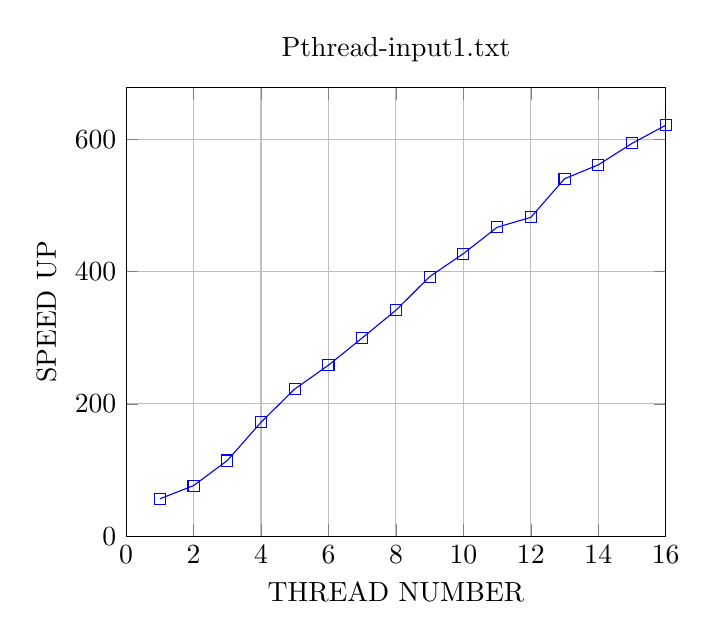
\begin{tikzpicture}
  \begin{axis}[
      title={Pthread-input1.txt},
      xlabel={THREAD NUMBER},
      ylabel={SPEED UP},
      xmin=0, xmax=16,
      ymajorgrids=true,
      xmajorgrids=true,
    ]
    \addplot[
      color=blue,
      mark=square,
    ]
      coordinates {
        (1  , 56.58818168426132  )
        (2  , 76.59159346794642  )
        (3  , 114.40169073656625 )
        (4  , 172.33644259905682 )
        (5  , 222.45999322712896 )
        (6  , 258.5117884515353  )
        (7  , 299.6500039427632  )
        (8  , 341.50738872666136 )
        (9  , 392.2434259525401  )
        (10 , 427.05118562894955 )
        (11 , 466.85340802987855 )
        (12 , 481.89856327893926 )
        (13 , 540.2166115514495  )
        (14 , 561.1697777131536  )
        (15 , 593.6386927451102  )
        (16 , 621.044612123696   )
      };
  \end{axis}
\end{tikzpicture}
\end{center}

\begin{center}
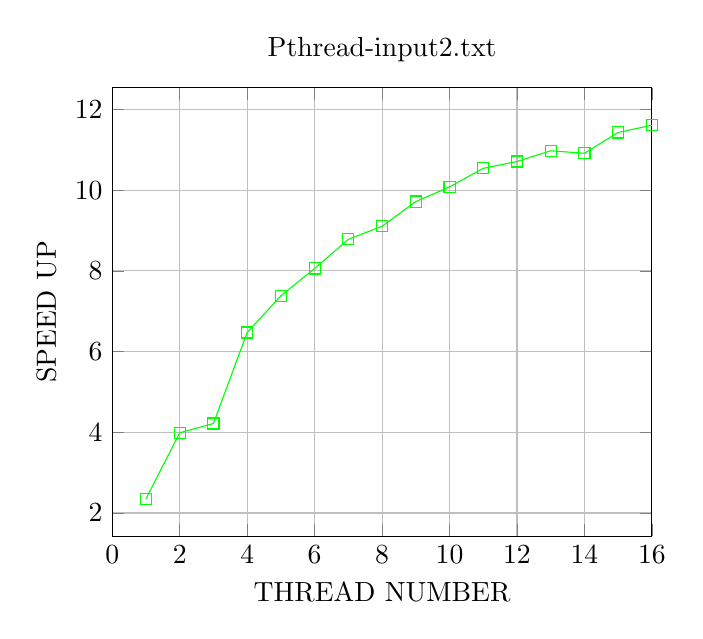
\begin{tikzpicture}
  \begin{axis}[
      title={Pthread-input2.txt},
      xlabel={THREAD NUMBER},
      ylabel={SPEED UP},
      xmin=0, xmax=16,
      ymajorgrids=true,
      xmajorgrids=true,
    ]
    \addplot[
      color=green,
      mark=square,
    ]
      coordinates {
        (1, 2.3519719268630808)
        (2, 3.988453995462279)
        (3, 4.218310843710378)
        (4, 6.4733418534842295)
        (5, 7.38200393988096)
        (6, 8.05998470905758)
        (7, 8.781834148789361)
        (8, 9.10566736736945)
        (9, 9.718011084085786)
        (10, 10.080470959603232)
        (11, 10.541438394328104)
        (12, 10.710471474954328)
        (13, 10.975778025865205)
        (14, 10.91403482512598)
        (15, 11.430512282901912)
        (16, 11.608970085342515)
      };
  \end{axis}
\end{tikzpicture}
\end{center}

\begin{center}
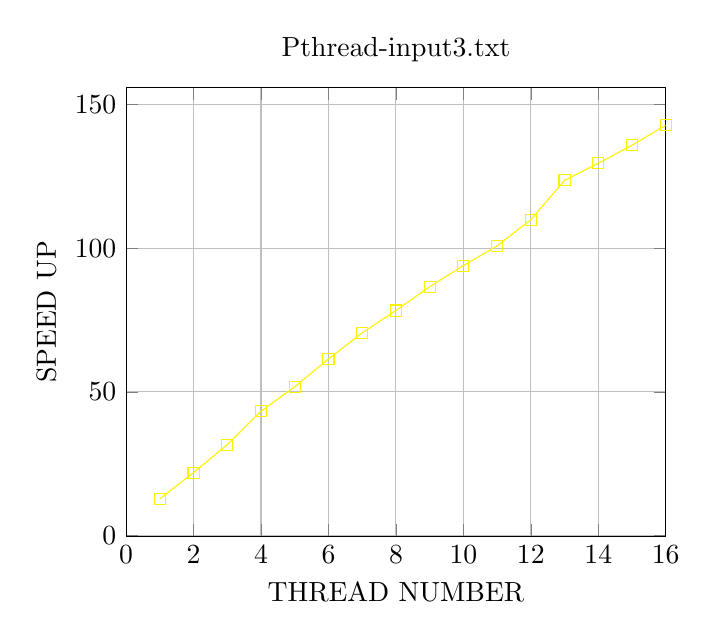
\begin{tikzpicture}
  \begin{axis}[
      title={Pthread-input3.txt},
      xlabel={THREAD NUMBER},
      ylabel={SPEED UP},
      xmin=0, xmax=16,
      ymajorgrids=true,
      xmajorgrids=true,
    ]
    \addplot[
      color=yellow,
      mark=square,
    ]
      coordinates {
        (1, 12.831703807539137)
        (2, 21.94624113398786)
        (3, 31.68305028080642)
        (4, 43.279391928968685)
        (5, 51.8062256463065)
        (6, 61.45099754196009)
        (7, 70.52704907038425)
        (8, 78.29662411856255)
        (9, 86.57196272271477)
        (10, 93.9136647262964)
        (11, 100.77331670951422)
        (12, 109.8967779343451)
        (13, 123.5400671512267)
        (14, 129.49817471131044)
        (15, 135.75791227096056)
        (16, 142.7101801387703)
      };
  \end{axis}
\end{tikzpicture}
\end{center}

三张图对应三个测试用例,其中横轴为可用线程数量,即处理器核,纵轴为加速比,
均使用了pthread。随着系统可用线程数量增加,加速比增大,在线程数量1至16的范
围内,加速比随线程数量几乎是线性增加(相同输入样例时)。不同测试样例的加速
比不同,其中样例2的加速比最低。

\subsection{加速比随自变量变化的趋势以及原因}
在相同测试样例时,加速比随可用线程数几乎线性增加,因为代码的实现方式中,字
符串长度决定了创建的线程数量,而字符串长度几乎远超可用线程数,所以每个处理
器核均可得到利用,当可用线程数量增加时,运行的线程也随之增加,加速比增大。

\section{结论}
\subsection{最佳优化方案与该方案优势}
最佳的优化方案是使用pthread按照子串长度划分任务。与使用openmp在二维表格对角
线上划分任务相比,该方法在运行过程中并行度会逐步增大,且不用依靠屏障同步数
据,能够及时地反馈数据变化与任务状态,而线程调度的任务则交由操作系统完成,
减少了调度和上下文切换带来的开销。

\end{document}
